%\section*{Appendix}




\begin{figure}[H]
  \centering
  \begin{subfigure}[b]{\textwidth}
  \centering
  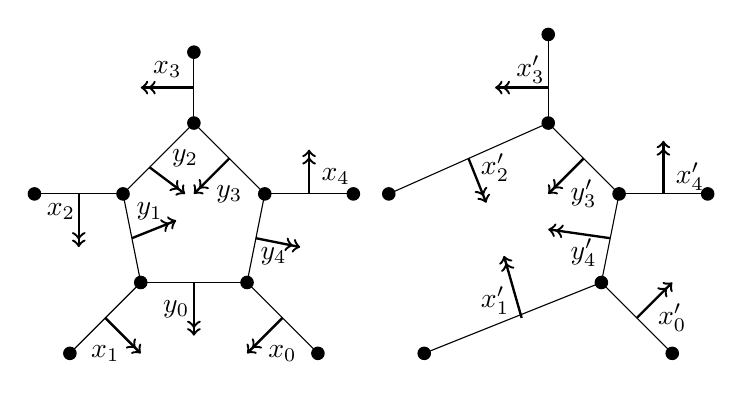
\begin{tikzpicture}[scale=0.45]
  \filldraw [black] (1.5,-1.5) circle (5pt);
%  \node[above left] at (1.5,-1.5) {$a_0$};
  \filldraw [black] (-1.5,-1.5) circle (5pt);
%  \node[above right] at (-1.5,-1.5) {$a_1$};
  \filldraw [black] (-2,1) circle (5pt);
%  \node[right] at (-2,1) {$a_2$};
  \filldraw [black] (2,1) circle (5pt);
%  \node[left] at (2,1) {$a_4$};
  \filldraw [black] (0,3) circle (5pt);
%  \node[below] at (0,3) {$a_3$};
  \filldraw [black] (3.5,-3.5) circle (5pt);
%  \node[right] at (3.5,-3.5) {$b_0$};
  \filldraw [black] (-3.5,-3.5) circle (5pt);
%  \node[left] at (-3.5,-3.5) {$b_1$};
  \filldraw [black] (-4.5,1) circle (5pt);
%  \node[left] at (-4.5,1) {$b_2$};
  \filldraw [black] (4.5,1) circle (5pt);
%  \node[right] at (4.5,1) {$b_4$};
  \filldraw [black] (0,5) circle (5pt);
%  \node[above] at (0,5.5) {$b_3$};
  \draw (1.5,-1.5) -- (-1.5,-1.5);
  \draw (-1.5, -1.5) -- (-2,1);
  \draw (-2,1) -- (0,3);
  \draw (0,3) -- (2,1);
  \draw (2,1) -- (1.5,-1.5);
  \draw (1.5,-1.5) -- (3.5,-3.5);
  \draw (-1.5,-1.5) -- (-3.5,-3.5);
  \draw (0,3) -- (0,5);
  \draw (-2,1) -- (-4.5,1);
  \draw (2,1) -- (4.5,1);
  \draw[->>, line width=0.3mm] (2.5, -2.5) -- (1.5,-3.5);
  \draw[->>, line width=0.3mm] (-2.5,-2.5) -- (-1.5,-3.5);
  \draw[->>, line width=0.3mm] (-3.25,1) -- (-3.25,-0.5);
  \draw[->>, line width=0.3mm] (0,4) -- (-1.5,4);
  \draw[->>, line width=0.3mm] (3.25,1) -- (3.25,2.25);
%  \node at (2.5,-3.5) {$x_0$};
%  \node at (-3.25,-2.5) {$x_1$};
%  \node at (-3.75,1.75) {$x_2$};
%  \node at (0.75,4.5) {$x_3$};
%  \node at (4,0.25) {$x_4$};
  \draw[->>, line width=0.3mm] (0,-1.5) -- (0,-3);
  \draw[->>, line width=0.3mm] (-1.75,-0.25) -- (-0.5,0.25);
  \draw[->>, line width=0.3mm] (1.75,-0.25) -- (3,-0.5);
  \draw[->>, line width=0.3mm] (-1.25,1.75) -- (-0.25,1);
  \draw[->>, line width=0.3mm] (1,2) -- (0,1);
  \node at (2.5,-3.5) {$x_0$};
  % \node at (-3.25,-2.5) {$x_1$};
  \node at (-2.5,-3.5) {$x_1$};
  % \node at (-3.75,1.75) {$x_2$};
  \node at (-3.75,0.5) {$x_2$};
  % \node at (0.75,4.5) {$x_3$};
  \node at (-0.75,4.5) {$x_3$};
  % \node at (4,0.25) {$x_4$};
  \node at (4,1.5) {$x_4$};
  \node at (-0.5,-2.25) {$y_0$};
  % \node at (-2.5,0) {$y_1$};
  \node at (-1.25,0.5) {$y_1$};
  % \node at (-1.25,2.5) {$y_2$};
  \node at (-0.25,2) {$y_2$};
  % \node at (2,2.25) {$y_3$};
  \node at (1,1) {$y_3$};
  \node at (2.25,-0.75) {$y_4$};
%  \node at (-0.5,-2.25) {$y_0$};
%  \node at (-2.5,0) {$y_1$};
%  \node at (-1.25,2.5) {$y_2$};
%  \node at (2,2.25) {$y_3$};
%  \node at (2.25,-0.75) {$y_4$};
  \filldraw [black] (11.5,-1.5) circle (5pt);
%  \node[above left] at (1.5,-1.5) {$a_0$};
  \filldraw [black] (12,1) circle (5pt);
%  \node[left] at (2,1) {$a_4$};
  \filldraw [black] (10,3) circle (5pt);
%  \node[below] at (0,3) {$a_3$};
  \filldraw [black] (13.5,-3.5) circle (5pt);
%  \node[right] at (3.5,-3.5) {$b_0$};
  \filldraw [black] (6.5,-3.5) circle (5pt);
%  \node[left] at (-3.5,-3.5) {$b_1$};
  \filldraw [black] (5.5,1) circle (5pt);
%  \node[left] at (-4.5,1) {$b_2$};
  \filldraw [black] (14.5,1) circle (5pt);
%  \node[right] at (4.5,1) {$b_4$};
  \filldraw [black] (10,5.5) circle (5pt);
%  \node[above] at (0,5.5) {$b_3$};
  \draw (10,3) -- (12,1);
  \draw (12,1) -- (11.5,-1.5);
  \draw (11.5,-1.5) -- (13.5,-3.5);
  \draw (10,3) -- (10,5.5);
  \draw (12,1) -- (14.5,1);
  \draw (6.5,-3.5) -- (11.5,-1.5); % b_1 -- a_0
  \draw (5.5,1) -- (10,3); % b_2 -- a_3
  \draw[->>, line width=0.3mm] (12.5, -2.5) -- (13.5,-1.5);
  \draw[->>, line width=0.3mm] (10,4) -- (8.5,4);
  \draw[->>, line width=0.3mm] (13.25,1) -- (13.25,2.5);
  \draw[->>, line width=0.3mm] (9.25,-2.5) -- (8.75,-0.75); % x'_1
  \draw[->>, line width=0.3mm] (7.75,2) -- (8.25,0.75); % x'_2
%  \node at (2.5,-3.35) {$x'_0$};
%  \node at (-2,-2.25) {$x'_1$};
%  \node at (-3.25,2.25) {$x'_2$};
%  \node at (0.75,4.65) {$x'_3$};
%  \node at (4,0.25) {$x'_4$};
  \draw[->>, line width=0.3mm] (11.75,-0.25) -- (10,0);
  \draw[->>, line width=0.3mm] (11,2) -- (10,1);
%  \node at (2,2.25) {$y'_3$};
%  \node at (2.25,-1) {$y'_4$};
  \node at (13.5,-2.5) {$x'_0$};
  \node at (8.5,-2) {$x'_1$};
  \node at (8.5,1.75) {$x'_2$};
  \node at (9.5,4.5) {$x'_3$};
  % \node at (4,0.25) {$x_4$};
  \node at (14,1.5) {$x'_4$};
  % \node at (2,2.25) {$y_3$};
  \node at (11,1) {$y'_3$};
  \node at (11,-0.65) {$y'_4$};
  \end{tikzpicture}
  \captionsetup{justification=centering}
  \caption{$(x'_0,x'_3,x'_4) = (0,0,0)$}
  \end{subfigure}
  

  \begin{subfigure}[b]{\textwidth}
  \centering
  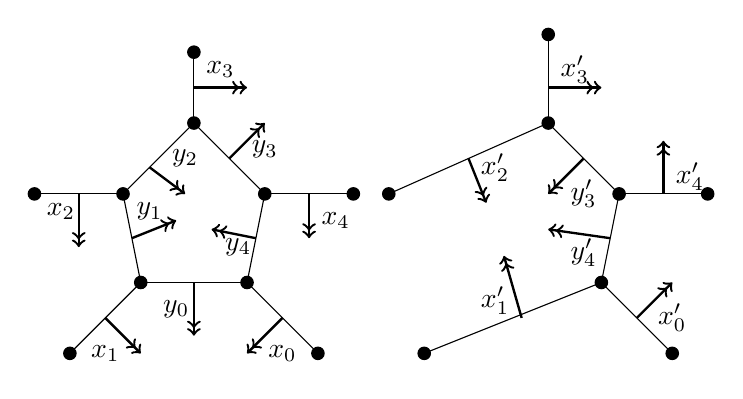
\begin{tikzpicture}[scale=0.45]
  \filldraw [black] (1.5,-1.5) circle (5pt);
%  \node[above left] at (1.5,-1.5) {$a_0$};
  \filldraw [black] (-1.5,-1.5) circle (5pt);
%  \node[above right] at (-1.5,-1.5) {$a_1$};
  \filldraw [black] (-2,1) circle (5pt);
%  \node[right] at (-2,1) {$a_2$};
  \filldraw [black] (2,1) circle (5pt);
%  \node[left] at (2,1) {$a_4$};
  \filldraw [black] (0,3) circle (5pt);
%  \node[below] at (0,3) {$a_3$};
  \filldraw [black] (3.5,-3.5) circle (5pt);
%  \node[right] at (3.5,-3.5) {$b_0$};
  \filldraw [black] (-3.5,-3.5) circle (5pt);
%  \node[left] at (-3.5,-3.5) {$b_1$};
  \filldraw [black] (-4.5,1) circle (5pt);
%  \node[left] at (-4.5,1) {$b_2$};
  \filldraw [black] (4.5,1) circle (5pt);
%  \node[right] at (4.5,1) {$b_4$};
  \filldraw [black] (0,5) circle (5pt);
%  \node[above] at (0,5.5) {$b_3$};
  \draw (1.5,-1.5) -- (-1.5,-1.5);
  \draw (-1.5, -1.5) -- (-2,1);
  \draw (-2,1) -- (0,3);
  \draw (0,3) -- (2,1);
  \draw (2,1) -- (1.5,-1.5);
  \draw (1.5,-1.5) -- (3.5,-3.5);
  \draw (-1.5,-1.5) -- (-3.5,-3.5);
  \draw (0,3) -- (0,5);
  \draw (-2,1) -- (-4.5,1);
  \draw (2,1) -- (4.5,1);
  \draw[->>, line width=0.3mm] (2.5, -2.5) -- (1.5,-3.5);
  \draw[->>, line width=0.3mm] (-2.5,-2.5) -- (-1.5,-3.5);
  \draw[->>, line width=0.3mm] (-3.25,1) -- (-3.25,-0.5);
  \draw[->>, line width=0.3mm] (0,4) -- (1.5,4);
  \draw[->>, line width=0.3mm] (3.25,1) -- (3.25,-0.25);
%  \node at (2.5,-3.5) {$x_0$};
%  \node at (-3.25,-2.5) {$x_1$};
%  \node at (-3.75,1.75) {$x_2$};
%  \node at (0.75,4.5) {$x_3$};
%  \node at (4,0.25) {$x_4$};
  \draw[->>, line width=0.3mm] (0,-1.5) -- (0,-3);
  \draw[->>, line width=0.3mm] (-1.75,-0.25) -- (-0.5,0.25);
  \draw[->>, line width=0.3mm] (1.75,-0.25) -- (0.5,0);
  \draw[->>, line width=0.3mm] (-1.25,1.75) -- (-0.25,1);
  \draw[->>, line width=0.3mm] (1,2) -- (2,3);
  \node at (2.5,-3.5) {$x_0$};
  % \node at (-3.25,-2.5) {$x_1$};
  \node at (-2.5,-3.5) {$x_1$};
  % \node at (-3.75,1.75) {$x_2$};
  \node at (-3.75,0.5) {$x_2$};
  \node at (0.75,4.5) {$x_3$};
  % \node at (-0.75,4.5) {$x_3$};
  \node at (4,0.25) {$x_4$};
  % \node at (4,1.5) {$x_4$};
  \node at (-0.5,-2.25) {$y_0$};
  % \node at (-2.5,0) {$y_1$};
  \node at (-1.25,0.5) {$y_1$};
  % \node at (-1.25,2.5) {$y_2$};
  \node at (-0.25,2) {$y_2$};
  \node at (2,2.25) {$y_3$};
  % \node at (1,1) {$y_3$};
  % \node at (2.25,-0.75) {$y_4$};
  \node at (1.25,-0.5) {$y_4$};
%  \node at (-0.5,-2.25) {$y_0$};
%  \node at (-2.5,0) {$y_1$};
%  \node at (-1.25,2.5) {$y_2$};
%  \node at (2,2.25) {$y_3$};
%  \node at (2.25,-0.75) {$y_4$};

  \filldraw [black] (11.5,-1.5) circle (5pt);
%  \node[above left] at (1.5,-1.5) {$a_0$};
  \filldraw [black] (12,1) circle (5pt);
%  \node[left] at (2,1) {$a_4$};
  \filldraw [black] (10,3) circle (5pt);
%  \node[below] at (0,3) {$a_3$};
  \filldraw [black] (13.5,-3.5) circle (5pt);
%  \node[right] at (3.5,-3.5) {$b_0$};
  \filldraw [black] (6.5,-3.5) circle (5pt);
%  \node[left] at (-3.5,-3.5) {$b_1$};
  \filldraw [black] (5.5,1) circle (5pt);
%  \node[left] at (-4.5,1) {$b_2$};
  \filldraw [black] (14.5,1) circle (5pt);
%  \node[right] at (4.5,1) {$b_4$};
  \filldraw [black] (10,5.5) circle (5pt);
%  \node[above] at (0,5.5) {$b_3$};
  \draw (10,3) -- (12,1);
  \draw (12,1) -- (11.5,-1.5);
  \draw (11.5,-1.5) -- (13.5,-3.5);
  \draw (10,3) -- (10,5.5);
  \draw (12,1) -- (14.5,1);
  \draw (6.5,-3.5) -- (11.5,-1.5); % b_1 -- a_0
  \draw (5.5,1) -- (10,3); % b_2 -- a_3
  \draw[->>, line width=0.3mm] (12.5, -2.5) -- (13.5,-1.5);
  \draw[->>, line width=0.3mm] (10,4) -- (11.5,4);
  \draw[->>, line width=0.3mm] (13.25,1) -- (13.25,2.5);
  \draw[->>, line width=0.3mm] (9.25,-2.5) -- (8.75,-0.75); % x'_1
  \draw[->>, line width=0.3mm] (7.75,2) -- (8.25,0.75); % x'_2
%  \node at (2.5,-3.35) {$x'_0$};
%  \node at (-2,-2.25) {$x'_1$};
%  \node at (-3.25,2.25) {$x'_2$};
%  \node at (0.75,4.65) {$x'_3$};
%  \node at (4,0.25) {$x'_4$};
  \draw[->>, line width=0.3mm] (11.75,-0.25) -- (10,0);
  \draw[->>, line width=0.3mm] (11,2) -- (10,1);
%  \node at (2,2.25) {$y'_3$};
%  \node at (2.25,-1) {$y'_4$};

  \node at (13.5,-2.5) {$x'_0$};
  \node at (8.5,-2) {$x'_1$};
  \node at (8.5,1.75) {$x'_2$};
  \node at (10.75,4.5) {$x'_3$};
  % \node at (4,0.25) {$x_4$};
  \node at (14,1.5) {$x'_4$};
  % \node at (2,2.25) {$y_3$};
  \node at (11,1) {$y'_3$};
  \node at (11,-0.65) {$y'_4$};
  \end{tikzpicture}
  \captionsetup{justification=centering}
  \caption{$(x'_0,x'_3,x'_4) = (0,1,0)$}
  \end{subfigure}
  
  
  \begin{subfigure}[b]{\textwidth}
  \centering
  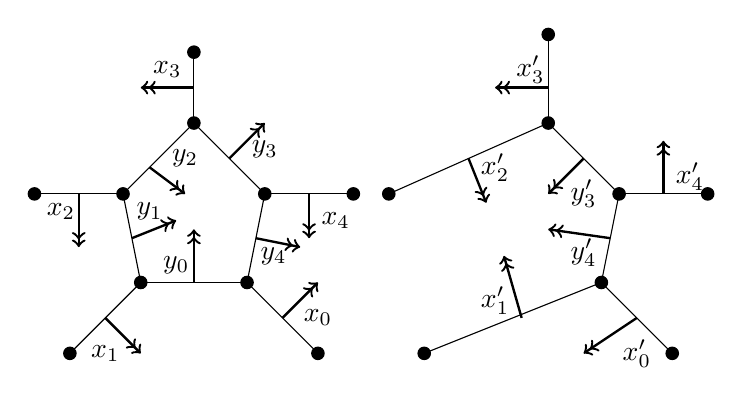
\begin{tikzpicture}[scale=0.45]
  \filldraw [black] (1.5,-1.5) circle (5pt);
%  \node[above left] at (1.5,-1.5) {$a_0$};
  \filldraw [black] (-1.5,-1.5) circle (5pt);
%  \node[above right] at (-1.5,-1.5) {$a_1$};
  \filldraw [black] (-2,1) circle (5pt);
%  \node[right] at (-2,1) {$a_2$};
  \filldraw [black] (2,1) circle (5pt);
%  \node[left] at (2,1) {$a_4$};
  \filldraw [black] (0,3) circle (5pt);
%  \node[below] at (0,3) {$a_3$};
  \filldraw [black] (3.5,-3.5) circle (5pt);
%  \node[right] at (3.5,-3.5) {$b_0$};
  \filldraw [black] (-3.5,-3.5) circle (5pt);
%  \node[left] at (-3.5,-3.5) {$b_1$};
  \filldraw [black] (-4.5,1) circle (5pt);
%  \node[left] at (-4.5,1) {$b_2$};
  \filldraw [black] (4.5,1) circle (5pt);
%  \node[right] at (4.5,1) {$b_4$};
  \filldraw [black] (0,5) circle (5pt);
%  \node[above] at (0,5.5) {$b_3$};
  \draw (1.5,-1.5) -- (-1.5,-1.5);
  \draw (-1.5, -1.5) -- (-2,1);
  \draw (-2,1) -- (0,3);
  \draw (0,3) -- (2,1);
  \draw (2,1) -- (1.5,-1.5);
  \draw (1.5,-1.5) -- (3.5,-3.5);
  \draw (-1.5,-1.5) -- (-3.5,-3.5);
  \draw (0,3) -- (0,5);
  \draw (-2,1) -- (-4.5,1);
  \draw (2,1) -- (4.5,1);
  \draw[->>, line width=0.3mm] (2.5, -2.5) -- (3.5,-1.5);
  \draw[->>, line width=0.3mm] (-2.5,-2.5) -- (-1.5,-3.5);
  \draw[->>, line width=0.3mm] (-3.25,1) -- (-3.25,-0.5);
  \draw[->>, line width=0.3mm] (0,4) -- (-1.5,4);
  \draw[->>, line width=0.3mm] (3.25,1) -- (3.25,-0.25);
%  \node at (2.5,-3.5) {$x_0$};
%  \node at (-3.25,-2.5) {$x_1$};
%  \node at (-3.75,1.75) {$x_2$};
%  \node at (0.75,4.5) {$x_3$};
%  \node at (4,0.25) {$x_4$};
  \draw[->>, line width=0.3mm] (0,-1.5) -- (0,0);
  \draw[->>, line width=0.3mm] (-1.75,-0.25) -- (-0.5,0.25);
  \draw[->>, line width=0.3mm] (1.75,-0.25) -- (3,-0.5);
  \draw[->>, line width=0.3mm] (-1.25,1.75) -- (-0.25,1);
  \draw[->>, line width=0.3mm] (1,2) -- (2,3);
  % \node at (2.5,-3.5) {$x_0$};
  \node at (3.5, -2.5) {$x_0$};
  % \node at (-3.25,-2.5) {$x_1$};
  \node at (-2.5,-3.5) {$x_1$};
  % \node at (-3.75,1.75) {$x_2$};
  \node at (-3.75,0.5) {$x_2$};
  % \node at (0.75,4.5) {$x_3$};
  \node at (-0.75,4.5) {$x_3$};
  \node at (4,0.25) {$x_4$};
  % \node at (4,1.5) {$x_4$};
  % \node at (-0.5,-2.25) {$y_0$};
  \node at (-0.5,-1) {$y_0$};
  % \node at (-2.5,0) {$y_1$};
  \node at (-1.25,0.5) {$y_1$};
  % \node at (-1.25,2.5) {$y_2$};
  \node at (-0.25,2) {$y_2$};
  \node at (2,2.25) {$y_3$};
  % \node at (1,1) {$y_3$};
  \node at (2.25,-0.75) {$y_4$};
%  \node at (-0.5,-2.25) {$y_0$};
%  \node at (-2.5,0) {$y_1$};
%  \node at (-1.25,2.5) {$y_2$};
%  \node at (2,2.25) {$y_3$};
%  \node at (2.25,-0.75) {$y_4$};

  \filldraw [black] (11.5,-1.5) circle (5pt);
%  \node[above left] at (1.5,-1.5) {$a_0$};
  \filldraw [black] (12,1) circle (5pt);
%  \node[left] at (2,1) {$a_4$};
  \filldraw [black] (10,3) circle (5pt);
%  \node[below] at (0,3) {$a_3$};
  \filldraw [black] (13.5,-3.5) circle (5pt);
%  \node[right] at (3.5,-3.5) {$b_0$};
  \filldraw [black] (6.5,-3.5) circle (5pt);
%  \node[left] at (-3.5,-3.5) {$b_1$};
  \filldraw [black] (5.5,1) circle (5pt);
%  \node[left] at (-4.5,1) {$b_2$};
  \filldraw [black] (14.5,1) circle (5pt);
%  \node[right] at (4.5,1) {$b_4$};
  \filldraw [black] (10,5.5) circle (5pt);
%  \node[above] at (0,5.5) {$b_3$};
  \draw (10,3) -- (12,1);
  \draw (12,1) -- (11.5,-1.5);
  \draw (11.5,-1.5) -- (13.5,-3.5);
  \draw (10,3) -- (10,5.5);
  \draw (12,1) -- (14.5,1);
  \draw (6.5,-3.5) -- (11.5,-1.5); % b_1 -- a_0
  \draw (5.5,1) -- (10,3); % b_2 -- a_3
  \draw[->>, line width=0.3mm] (12.5, -2.5) -- (11,-3.5);
  \draw[->>, line width=0.3mm] (10,4) -- (8.5,4);
  \draw[->>, line width=0.3mm] (13.25,1) -- (13.25,2.5);
  \draw[->>, line width=0.3mm] (9.25,-2.5) -- (8.75,-0.75); % x'_1
  \draw[->>, line width=0.3mm] (7.75,2) -- (8.25,0.75); % x'_2
%  \node at (2.5,-3.35) {$x'_0$};
%  \node at (-2,-2.25) {$x'_1$};
%  \node at (-3.25,2.25) {$x'_2$};
%  \node at (0.75,4.65) {$x'_3$};
%  \node at (4,0.25) {$x'_4$};
  \draw[->>, line width=0.3mm] (11.75,-0.25) -- (10,0);
  \draw[->>, line width=0.3mm] (11,2) -- (10,1);
%  \node at (2,2.25) {$y'_3$};
%  \node at (2.25,-1) {$y'_4$};
  \node at (12.5,-3.5) {$x'_0$};
  \node at (8.5,-2) {$x'_1$};
  \node at (8.5,1.75) {$x'_2$};
  \node at (9.5,4.5) {$x'_3$};
  % \node at (4,0.25) {$x_4$};
  \node at (14,1.5) {$x'_4$};
  % \node at (2,2.25) {$y_3$};
  \node at (11,1) {$y'_3$};
  \node at (11,-0.65) {$y'_4$};
  \end{tikzpicture}
  \captionsetup{justification=centering}
  \caption{$(x'_0,x'_3,x'_4) = (1,0,0)$}
  \end{subfigure}
  
  
  \begin{subfigure}[b]{\textwidth}
  \centering
  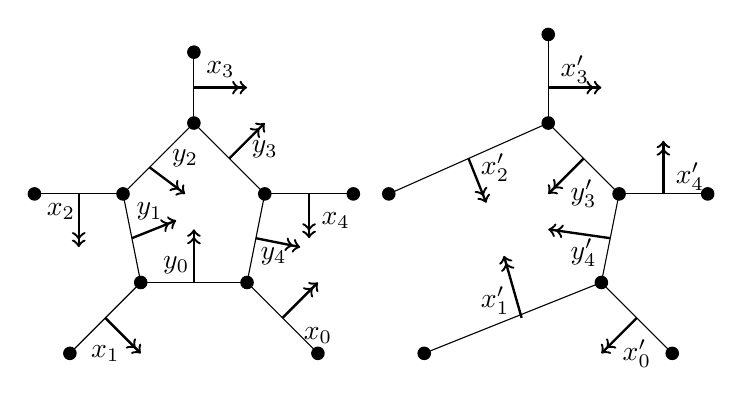
\begin{tikzpicture}[scale=0.45]
  \filldraw [black] (1.5,-1.5) circle (5pt);
%  \node[above left] at (1.5,-1.5) {$a_0$};
  \filldraw [black] (-1.5,-1.5) circle (5pt);
%  \node[above right] at (-1.5,-1.5) {$a_1$};
  \filldraw [black] (-2,1) circle (5pt);
%  \node[right] at (-2,1) {$a_2$};
  \filldraw [black] (2,1) circle (5pt);
%  \node[left] at (2,1) {$a_4$};
  \filldraw [black] (0,3) circle (5pt);
%  \node[below] at (0,3) {$a_3$};
  \filldraw [black] (3.5,-3.5) circle (5pt);
%  \node[right] at (3.5,-3.5) {$b_0$};
  \filldraw [black] (-3.5,-3.5) circle (5pt);
%  \node[left] at (-3.5,-3.5) {$b_1$};
  \filldraw [black] (-4.5,1) circle (5pt);
%  \node[left] at (-4.5,1) {$b_2$};
  \filldraw [black] (4.5,1) circle (5pt);
%  \node[right] at (4.5,1) {$b_4$};
  \filldraw [black] (0,5) circle (5pt);
%  \node[above] at (0,5.5) {$b_3$};
  \draw (1.5,-1.5) -- (-1.5,-1.5);
  \draw (-1.5, -1.5) -- (-2,1);
  \draw (-2,1) -- (0,3);
  \draw (0,3) -- (2,1);
  \draw (2,1) -- (1.5,-1.5);
  \draw (1.5,-1.5) -- (3.5,-3.5);
  \draw (-1.5,-1.5) -- (-3.5,-3.5);
  \draw (0,3) -- (0,5);
  \draw (-2,1) -- (-4.5,1);
  \draw (2,1) -- (4.5,1);
  \draw[->>, line width=0.3mm] (2.5, -2.5) -- (3.5,-1.5);
  \draw[->>, line width=0.3mm] (-2.5,-2.5) -- (-1.5,-3.5);
  \draw[->>, line width=0.3mm] (-3.25,1) -- (-3.25,-0.5);
  \draw[->>, line width=0.3mm] (0,4) -- (1.5,4);
  \draw[->>, line width=0.3mm] (3.25,1) -- (3.25,-0.25);
%  \node at (2.5,-3.5) {$x_0$};
%  \node at (-3.25,-2.5) {$x_1$};
%  \node at (-3.75,1.75) {$x_2$};
%  \node at (0.75,4.5) {$x_3$};
%  \node at (4,0.25) {$x_4$};
  \draw[->>, line width=0.3mm] (0,-1.5) -- (0,0);
  \draw[->>, line width=0.3mm] (-1.75,-0.25) -- (-0.5,0.25);
  \draw[->>, line width=0.3mm] (1.75,-0.25) -- (3,-0.5);
  \draw[->>, line width=0.3mm] (-1.25,1.75) -- (-0.25,1);
  \draw[->>, line width=0.3mm] (1,2) -- (2,3);
  % \node at (2.5,-3.5) {$x_0$};
  \node at (3.5,-3) {$x_0$};
  % \node at (-3.25,-2.5) {$x_1$};
  \node at (-2.5,-3.5) {$x_1$};
  % \node at (-3.75,1.75) {$x_2$};
  \node at (-3.75,0.5) {$x_2$};
  % \node at (0.75,4.5) {$x_3$};
  \node at (0.75,4.5) {$x_3$};
  \node at (4,0.25) {$x_4$};
  % \node at (4,1.5) {$x_4$};
  % \node at (-0.5,-2.25) {$y_0$};
  \node at (-0.5, -1) {$y_0$};
  % \node at (-2.5,0) {$y_1$};
  \node at (-1.25,0.5) {$y_1$};
  % \node at (-1.25,2.5) {$y_2$};
  \node at (-0.25,2) {$y_2$};
  \node at (2,2.25) {$y_3$};
  % \node at (1,1) {$y_3$};
  \node at (2.25,-0.75) {$y_4$};
%  \node at (-0.5,-2.25) {$y_0$};
%  \node at (-2.5,0) {$y_1$};
%  \node at (-1.25,2.5) {$y_2$};
%  \node at (2,2.25) {$y_3$};
%  \node at (2.25,-0.75) {$y_4$};

  \filldraw [black] (11.5,-1.5) circle (5pt);
%  \node[above left] at (1.5,-1.5) {$a_0$};
  \filldraw [black] (12,1) circle (5pt);
%  \node[left] at (2,1) {$a_4$};
  \filldraw [black] (10,3) circle (5pt);
%  \node[below] at (0,3) {$a_3$};
  \filldraw [black] (13.5,-3.5) circle (5pt);
%  \node[right] at (3.5,-3.5) {$b_0$};
  \filldraw [black] (6.5,-3.5) circle (5pt);
%  \node[left] at (-3.5,-3.5) {$b_1$};
  \filldraw [black] (5.5,1) circle (5pt);
%  \node[left] at (-4.5,1) {$b_2$};
  \filldraw [black] (14.5,1) circle (5pt);
%  \node[right] at (4.5,1) {$b_4$};
  \filldraw [black] (10,5.5) circle (5pt);
%  \node[above] at (0,5.5) {$b_3$};
  \draw (10,3) -- (12,1);
  \draw (12,1) -- (11.5,-1.5);
  \draw (11.5,-1.5) -- (13.5,-3.5);
  \draw (10,3) -- (10,5.5);
  \draw (12,1) -- (14.5,1);
  \draw (6.5,-3.5) -- (11.5,-1.5); % b_1 -- a_0
  \draw (5.5,1) -- (10,3); % b_2 -- a_3
  \draw[->>, line width=0.3mm] (12.5, -2.5) -- (11.5,-3.5);
  \draw[->>, line width=0.3mm] (10,4) -- (11.5,4);
  \draw[->>, line width=0.3mm] (13.25,1) -- (13.25,2.5);
  \draw[->>, line width=0.3mm] (9.25,-2.5) -- (8.75,-0.75); % x'_1
  \draw[->>, line width=0.3mm] (7.75,2) -- (8.25,0.75); % x'_2
%  \node at (2.5,-3.35) {$x'_0$};
%  \node at (-2,-2.25) {$x'_1$};
%  \node at (-3.25,2.25) {$x'_2$};
%  \node at (0.75,4.65) {$x'_3$};
%  \node at (4,0.25) {$x'_4$};
  \draw[->>, line width=0.3mm] (11.75,-0.25) -- (10,0);
  \draw[->>, line width=0.3mm] (11,2) -- (10,1);
%  \node at (2,2.25) {$y'_3$};
%  \node at (2.25,-1) {$y'_4$};
  \node at (12.5,-3.5) {$x'_0$};
  \node at (8.5,-2) {$x'_1$};
  \node at (8.5,1.75) {$x'_2$};
  \node at (10.75,4.5) {$x'_3$};
  % \node at (4,0.25) {$x_4$};
  \node at (14,1.5) {$x'_4$};
  % \node at (2,2.25) {$y_3$};
  \node at (11,1) {$y'_3$};
  \node at (11,-0.65) {$y'_4$};
  \end{tikzpicture}
  \captionsetup{justification=centering}
  \caption{$(x'_0,x'_3,x'_4) = (1,1,0)$}
  \end{subfigure}
  \captionsetup{justification=centering}
  \caption{Geometric picture in the proof of Theorem \ref{thm:P3EM}}
  \label{geometry}
\end{figure}

\newpage







% \begin{figure}[ht]
%   \centering
% %  \begin{subfigure}[b]{0.4\textwidth}
% %  \centering
%   \begin{tikzpicture}[scale=0.5]
%   \node at (0,0.5) {$P$};
%   \filldraw [black] (1.5,-1.5) circle (5pt);
%   \node[above left] at (1.5,-1.5) {$a_0$};
%   \filldraw [black] (-1.5,-1.5) circle (5pt);
%   \node[above right] at (-1.5,-1.5) {$a_1$};
%   \filldraw [black] (-2,1) circle (5pt);
%   \node[right] at (-2,1) {$a_2$};
%   \filldraw [black] (2,1) circle (5pt);
%   \node[left] at (2,1) {$a_4$};
%   \filldraw [black] (0,3) circle (5pt);
%   \node[below] at (0,3) {$a_3$};
%   \filldraw [black] (-2.5,-2.5) circle (5pt);
%   \node[above] at (-2.5,-2.5) {$b_1$};
%   \filldraw [black] (3.5,1) circle (5pt);
%   \node[right] at (3.5,1) {$b_4$};
%   \filldraw [black] (0,4.5) circle (5pt);
%   \node[above] at (0,4.5) {$b_3$};
%   \filldraw [black] (2,5) circle (5pt);
%   \node[below] at (2,5) {$b_0=b_2$};
%   \draw (1.5,-1.5) -- (-1.5,-1.5);
%   \draw (-1.5, -1.5) -- (-2,1);
%   \draw (-2,1) -- (0,3);
%   \draw (0,3) -- (2,1);
%   \draw (2,1) -- (1.5,-1.5);
%   \draw[thick] (-1.5,-1.5) -- (-2.5,-2.5);
%   \draw[thick] (0,3) -- (0,4.5);
%   \draw[thick] (2,1) -- (3.5,1);
%   \draw (-2,1) .. controls (-3,8) and (0,8) .. (2,5);
%   \draw (1.5,-1.5) .. controls (6,-2) and (7,6) .. (2,5);
%   \draw[thick, red] (2,5) -- (3.5,6.5);
%   \draw[thick, dotted] (0,4.5) -- (1,5.5);
%   \draw[thick, dotted] (0,4.5) -- (1,3.5);
%   \draw[thick, dotted] (3.5,1) -- (2.5,2);
%   \draw[thick, dotted] (3.5,1) -- (4.5,2);
%   \draw[thick, dotted] (-2.5,-2.5) -- (-3.5,-2.5);
%   \draw[thick, dotted] (-2.5,-2.5) -- (-2.5,-3.5);
%   \end{tikzpicture}  
%   \captionsetup{justification=centering}
%    \caption{Pentagon with red edge}
%    \label{trouble}
% \end{figure}